
\setlength{\parskip}{1em}   

\section*{Conference site plan}

\begin{figure}[H]
	\centering
	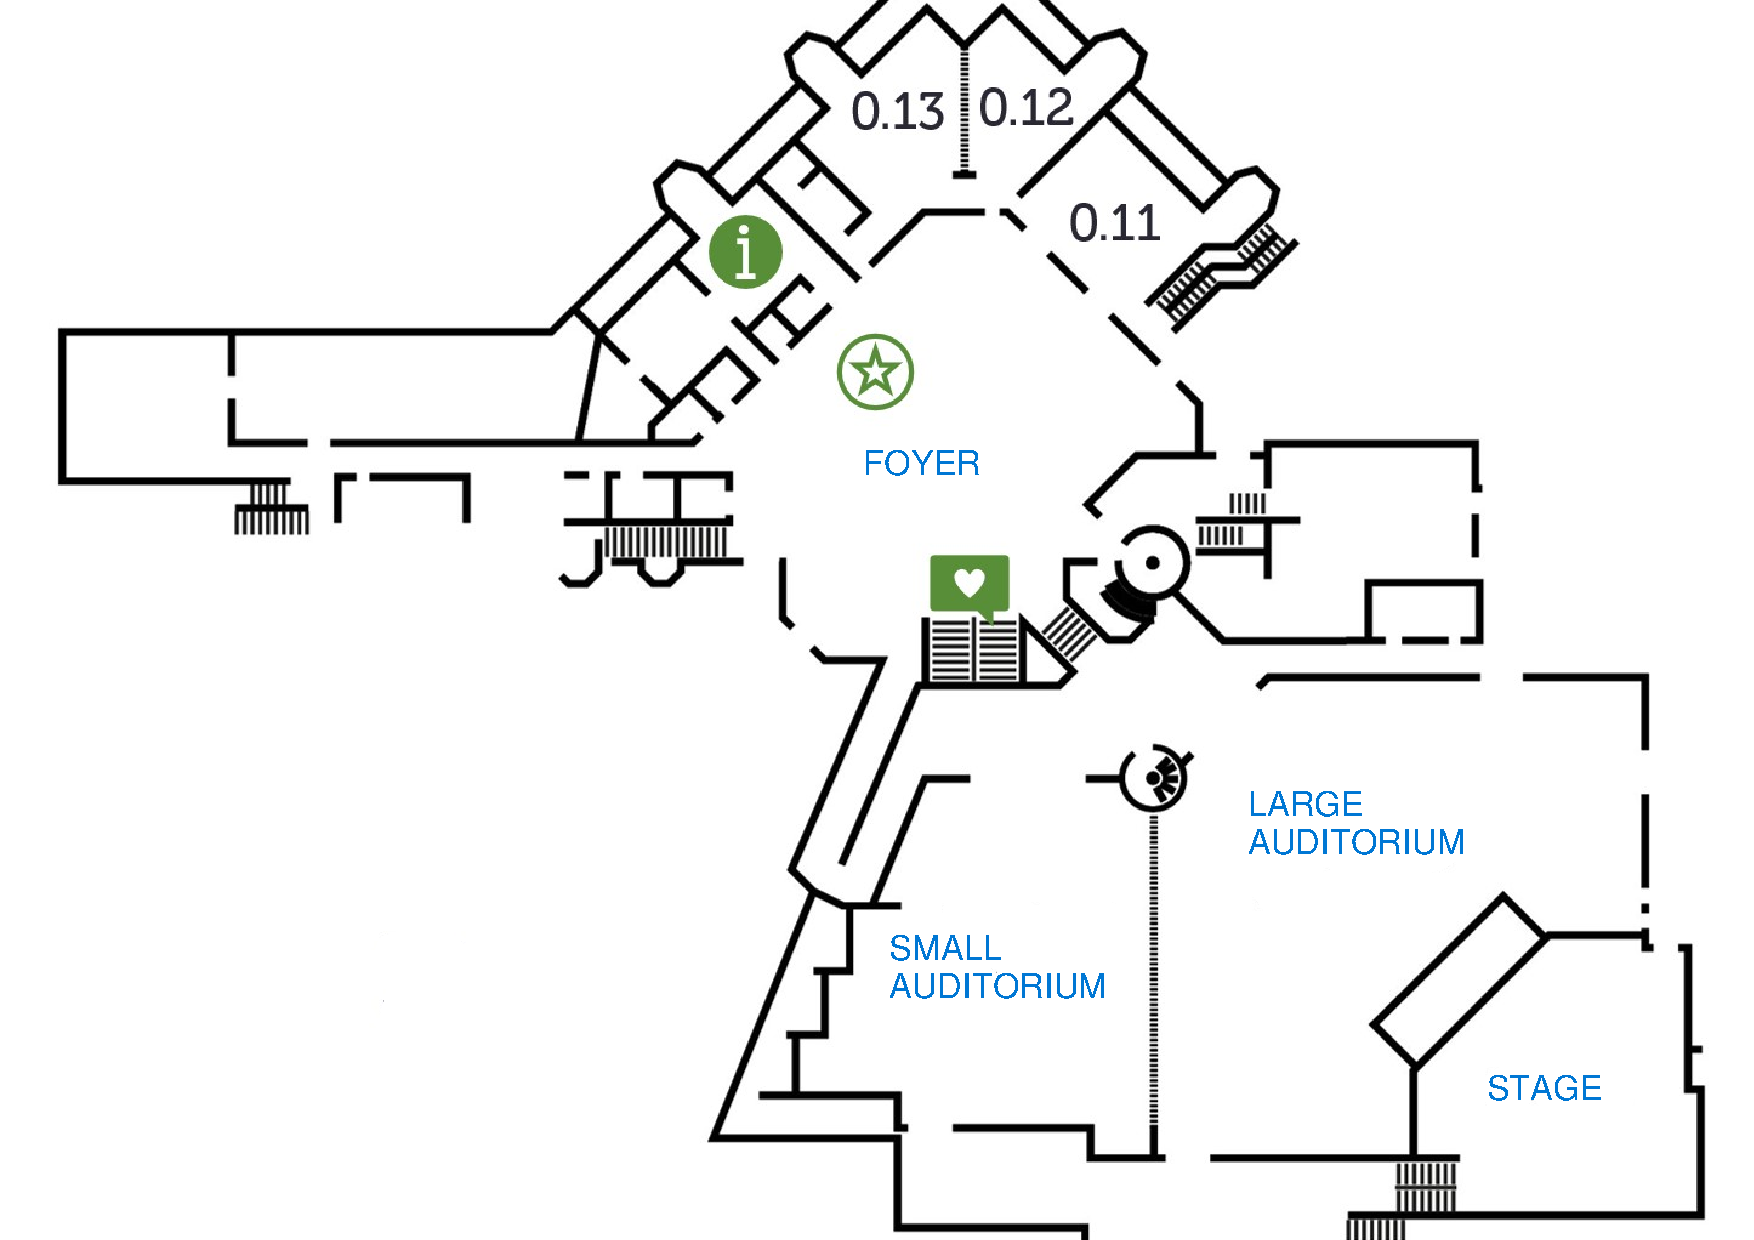
\includegraphics[width=0.7\textwidth]{pdf_static/ground_floor.pdf}
	\caption*{GROUND FLOOR}
	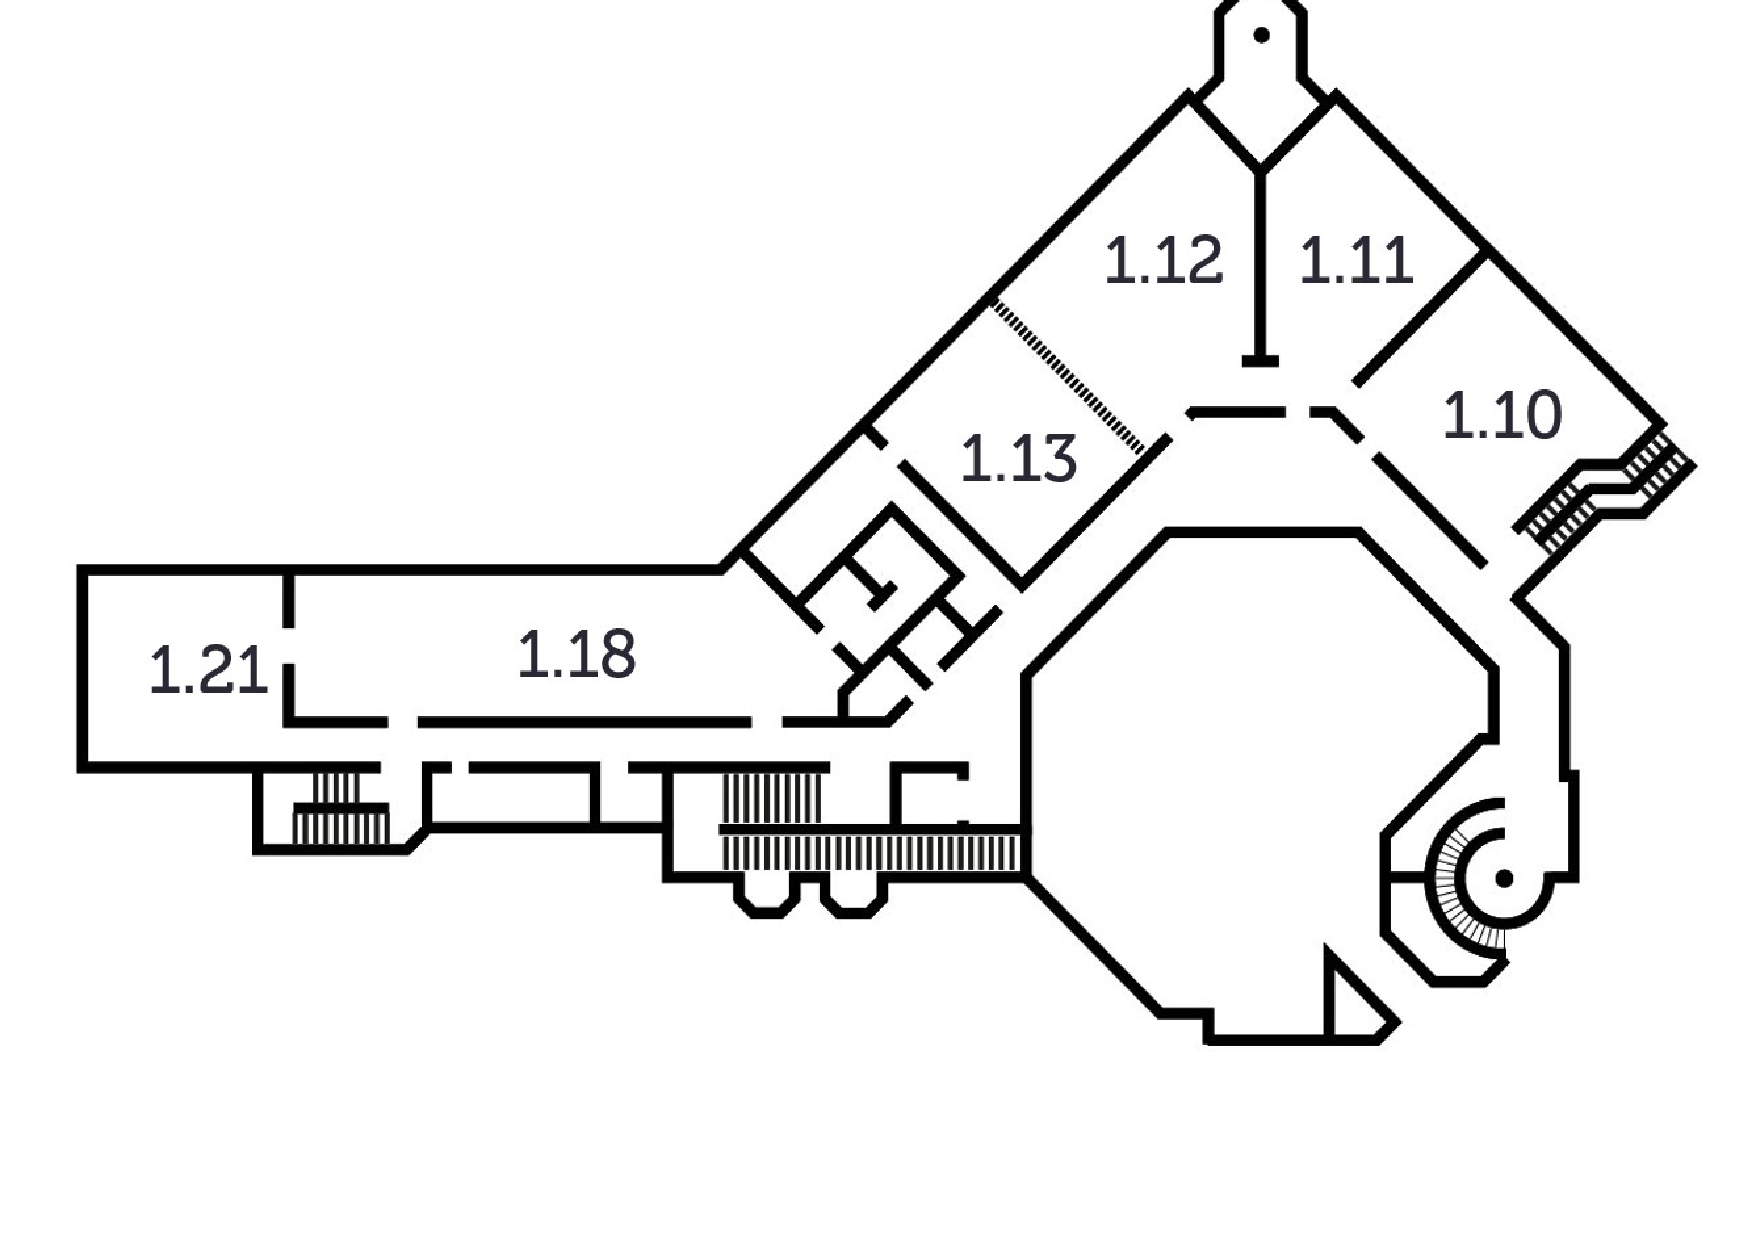
\includegraphics[width=0.7\textwidth]{pdf_static/first_floor.pdf}
	\caption*{FIRST FLOOR}
\end{figure}


\section*{How do I get to the venue?}

The Bürgerhaus Wilhelmsburg (Mengestraße 20, 21107 Hamburg) is a 12-min walk from Wilhelmsburg train station that can be reached via S-Bahn lines 3 and 5 (from the city center in the direction of Hamburg Neugraben and Stade/Buxtehude, respectively). Trains leave every 5-10 minutes. 
The bus station Rathaus Wilhelmsburg is right next to the venue. The bus 13 (sometimes also 152 and 154) go there from the train station.
Limited free parking is also available.

We recommend the HVV- and Stadtrad-Apps for getting around in Hamburg.

\begin{figure}[H]
	\centering
	\includegraphics[width=0.9\textwidth]{tex/images/infos/venue_path.png}
\end{figure}


%\section*{Accreditation}

% Four symposia have been accredited by the Landespsychotherapeutenkammer Baden-Württembergwith with 2 credit points each. If you need a certificate of participation, ask our staff in the respective symposium session: 

% \begin{itemize}
% \setlength{\itemsep}{-0.8em} 
% 	\item S04 - Neurobiological Research to Optimize Therapeutic Interventions
% 	\item S16 - Computational Mechanisms of Learning and Decision-making in Psychiatry
% 	\item S20 - Prefrontal Cortical Function and Neuromodulation in Mental Disorders
% 	\item S36 - Deficits in Tactile Perception and their Clinical Implications
% \end{itemize}

\vspace*{1cm}

\section*{Childcare}

There will be a range of qualified educators on site to look after children aged three and over. This service is free of charge. If you are interested in this offer, please contact us via email. The subject of the email should be: Childcare. 
You can reach us at pug2024@uni-hamburg.de

% \section*{How do I get to the social evening? And how do I get home later at night?}

% The Brauwerk Freistil is located south of the Neckar and easily reachable from the main station or Neckarbrücke within 10 minutes by foot.

% \begin{center}
% \includegraphics[width=1\textwidth]{tex/images/freistil.png}
% \end{center}


% Tübingen has a few night busses that run until 3 am. They are marked with an “N”. Alternatively, there are a few taxi companies:

% \begin{itemize}
% \setlength{\itemsep}{-0.8em} 
% 	\item Taxi Tübingen 07071 920555 and 0157 80989740
% 	\item Taxi Akublut 07071 1438591
% 	\item Taxi Maxi Tübingen 07071 7931064
% 	\item Taxi Easy 0173 1643229
% \end{itemize}


% \section*{What is a good place to eat and drink in Hamburg?}

% Tübingen has a few nice cafés, restaurants and bars to offer. Coffee places with a nice atmosphere are Café Haag, Café Hanseatica, Willi Tübingen, Suedhang Kaffee and Katesch.
% For authentic Swabian food, we recommend Krumme Brücke, Mauganeschtle, Marquardtei, Weinstube Forelle, Ratskeller and Wurstküche. The Neckarmüller is a nice beergarden and the Bären serves Swabian tapas! The Bären and Ratskeller are nice places to stay for one or a few more beers. Other good bars are the Jäger, Stadtpost, Chez Michel and the Irish pub Saints and Scholars.


% \section*{And if I need money?}

% Contactless payment is available almost everywhere, but some bars still rely on cash. You can find the nearest ATM close to the venue at the BG Klinik at Schnarrenbergstraße.

% \begin{center}
% \includegraphics[width=0.8\textwidth]{tex/images/atm.png}
% \end{center}


% We hope that this information will make your stay as pleasant as possible and that you will enjoy the PuG in Hamburg to the fullest!

